\documentclass{article}

\usepackage[a4paper, total={6in, 10in}, includeheadfoot]{geometry}
\usepackage[german]{babel}
\usepackage{pgfplots}
\usepackage{hyperref}
\usepackage{graphicx}
\usepackage{longtable}
\usepackage[utf8]{inputenc}

\graphicspath{ {./assets/} }
\pgfplotsset{compat=1.16}
\urlstyle{same}
\hypersetup{
    colorlinks=true,
    linkcolor=black,
    filecolor=blue,      
    urlcolor=blue,
}

\begin{document}
\selectlanguage{german}

\title{\vspace{-2cm}TI3 Web-Technologie: Case-Study 1}
\author{Sven Gehring, André Glatzl}
\date{}
\maketitle

\begin{abstract}
\noindent
Dieses Dokument dient als organisatorische und technische Dokumentation der IBZ Web-Technologie Case-Study 1. Ziel der Case-Study, gemäss Vorgabe, ist die Durchführung eines Projekts zur Entwicklung eines einfachen, webbasierenden Tagebuchsystems.

\vspace{5mm}
\noindent
Da alle Teilnehmer dieser Case-Study bereits über Vorwissen im entsprechenden Bereich verfügen und die technische Umsetzung der Anforderungen daher relativ trivial erscheint, fokusiert sich diese Case-Study vor allem auf die organisatorischen und dokumentarischen Aspekte eines Entwicklungsprojekts.

\vspace{5mm}
\noindent
Als nennenswerte selbst gesteckte Ziele wurde deshalb festgelegt, diese Dokumentation komplett in \LaTeX zu schreiben, um sich mit dieser Technologie für zukünftige Arbeiten vertraut zu machen. Zudem soll der geschriebene PHP Code komplett nach dem \emph{Test-Driven-Development} Prinzip programmiert werden, um das Wissen in diesem Bereich zu vertiefen und auf die für PHP verfügbaren Tools auszuweiten.

\end{abstract}

% TODO: Remove this for final version!
\begin{center}
  \textcolor{red}{\textbf{\emph{!Unvollständige Fassung für Zwischentermine!}}}
\end{center}

\tableofcontents

% Imported document contents
\clearpage
\section{Projektplanung}
\subsection{Projektziele}
Nachfolgend werden die relevanten Projektziele aufgelistet. Die Ziele sind dabei nach Stakeholder unterteilt und bestehen aus den funktionalen Anforderungen (FA), sowie den nicht-funktionalen Anforderungen (NFA) der Case-Study, und zusätzlichen Zielen, welche sich aus den restlichen Stakeholdern ergeben.
Die Ziele sind nachfolgend in Muss- (\textbf{M}) und Wunschziele (\textbf{W}) eingeteilt.

\vspace{5mm}

\begin{longtable}{ p{2.2cm}|p{10cm}|c|c  }
    \textbf{Stakeholder} & \textbf{Ziel} & \textbf{M} & \textbf{W} \\
    \hline
    Benutzer & FA\_1.1 Tagebucheinträge müssen erfasst werden können & x & \\
    & FA\_1.2 Jeder Tagebucheintrag hat ein auswählbares Datum & x & \\
    & FA\_1.3 Jeder Tagebucheintrag kann einer Kategorie zugeordnet werden & x & \\
    & FA\_1.4 Zu jedem Eintrag kann ein Freitext inkl. Sonderzeichen von bis zu 1000 Zeichen erfasst werden. & x & \\
    & FA\_1.5 Zu jedem Eintrag kann ein Bild erfasst werden. & & 3 \\
    & FA\_1.8 Einträge können nach Datum gefiltert werden. & & 4 \\
    & FA\_1.9 Einträge können nach Kategorie gefiltert werden. & & 4 \\
    & FA\_1.10 Es kann abgefragt werden, für welche Tage keine Tagebucheinträge vorhanden sind. & & 3 \\
    & FA\_1.11 Das Tagebuch ist mit einem Login geschützt. & x & \\
    & FA\_1.12 Ein Nutzer kann sich ein Login erstellen. & x & \\
    & NFA\_1.1 Das Tagebuch ist für unerfahrene Nutzer intuitiv zu bedienen & & 5 \\
    & NFA\_1.2 Das Tagebuch soll ein zeitgemässes Design besitzen & & 4 \\
    Sysadmin & FA\_1.6 Jeder Tagebucheintrag wird in der Datenbank gespeichert. &x & \\
    & FA\_1.7 Die Kategorien sind in der Datenbank gespeichert. & x& \\
    & FA\_1.13 Jeder User sieht nur seine eigenen Einträge & x & \\
    & NFA\_1.3 Das Tagebuch ist unter Windows und Linux lauffähig & & 4 \\
    & NFA\_1.4 Die Antwortszeigt des Tagebuchs liegt unter 3s & & 4 \\
    & NFA\_1.5 Das Tagebuch muss online sein & x & \\
    & Passwörter werden sicher gespeichert (PBKDF2 hash) & & 5 \\
    Entwickler & Die Dokumentation soll in \LaTeX geschrieben werden & & 3 \\
    & Es soll Versionskontrolle mit Git verwendet werden & & 5 \\
    Reviewer & Tests sollen in der Dokumentation ersichtlich sein & & 4 \\
    & Das gewählte System muss einfach erweiterbar sein & & 5 \\
    & Aktuelle Revision soll auf der Seite angezeigt werden & & 5 \\
    & ERM und Klassendiagramm soll verfügbar sein & & 4 \\
\end{longtable}

\noindent
Nachfolgend werden die aufgestellten Ziele in verschiedene Kategorien eingeteilt, um die Lösungsfindung zu veranschaulichten. Hierbei ist anzumerken, dass durch das Agile Projektmanagement die Lösungsfindung eher oberflächlich ausfällt und detaillierte Entscheidungen erst beim Grooming der jeweiligen User-Story gefällt wurden.

Die Ziele werden dabei in die Kategorien Framework (\textbf{F}), Sicherheit (\textbf{S}), Erfassung (\textbf{E}) Management (\textbf{M}) und Projekt (\textbf{P}) eingeteilt

\begin{longtable}{ p{10cm}ccccc }
    \textbf{Ziel} & \textbf{F} & \textbf{S} & \textbf{E} & \textbf{M} & \textbf{P} \\
    \hline
    FA\_1.1 Tagebucheinträge müssen erfasst werden können &&&x& \\
    FA\_1.2 Jeder Tagebucheintrag hat ein auswählbares Datum &&&x& \\
    FA\_1.3 Jeder Tagebucheintrag kann einer Kategorie zugeordnet werden &&&x& \\
    FA\_1.4 Zu jedem Eintrag kann ein Freitext inkl. Sonderzeichen von bis zu 1000 Zeichen erfasst werden. &&&x& \\
    FA\_1.5 Zu jedem Eintrag kann ein Bild erfasst werden. &&&x& \\
    FA\_1.8 Einträge können nach Datum gefiltert werden. &&&&x \\
    FA\_1.9 Einträge können nach Kategorie gefiltert werden. &&&&x \\
    FA\_1.10 Es kann abgefragt werden, für welche Tage keine Tagebucheinträge vorhanden sind. &&&&x \\
    FA\_1.11 Das Tagebuch ist mit einem Login geschützt. &&x&& \\
    FA\_1.12 Ein Nutzer kann sich ein Login erstellen. &&x&& \\
    NFA\_1.1 Tagebuch ist für unerfahrene Nutzer intuitiv zu bedienen &x&&& \\
    NFA\_1.2 Das Tagebuch soll ein zeitgemässes Design besitzen &x&&& \\
    FA\_1.6 Jeder Tagebucheintrag wird in der Datenbank gespeichert. &&&x& \\
    FA\_1.7 Die Kategorien sind in der Datenbank gespeichert. &&&x& \\
    FA\_1.13 Jeder User sieht nur seine eigenen Einträge &&x&& \\
    NFA\_1.3 Das Tagebuch ist unter Windows und Linux lauffähig &x&&& \\
    NFA\_1.4 Die Antwortszeigt des Tagebuchs liegt unter 3s &x&&& \\
    NFA\_1.5 Das Tagebuch muss online sein &x&&& \\
    Passwörter werden sicher gespeichert (PBKDF2 hash) &&x&& \\
    Die Dokumentation soll in \LaTeX geschrieben werden &&&&&x \\
    Es soll Versionskontrolle mit Git verwendet werden &&&&&x \\
    Das gewählte System muss einfach erweiterbar sein &x&&&& \\
    Tests sollen in der Dokumentation ersichtlich sein &&&&&x \\
    Aktuelle Revision soll auf der Seite angezeigt werden &&&&&x \\
    ERM und Klassendiagramm soll verfügbar sein &&&&&x \\
\end{longtable}
\subsection{Projektmanagement}
Für die Planung und Durchführung der Case-Study wird eine agile Vorgehensweise nach SCRUM gewählt. Der Sprint-Zyklus wird hierbei auf \emph{2 Wochen} festgelegt. Ein Sprint an sich dauert 12 Tage, zudem befinden sich zwischen zwei Sprints jeweils 2 freie Tage, an denen Sprint-Review und Sprint-Retrospect durchgeführt werden können.

Bedingt durch die fixen Termine der Case-Study, wurde die Arbeitszeit in \emph{6 Sprints} unterteilt. Damit die Sprints als konstante Zeiteinheit repräsentativ für Schätzungen sind, obwohl die Case-Study nebst Studium und Beruf durchgeführt wird, wird jedem Sprint ein fixes Zeitbudget von \emph{13 Lektionen pro Teilnehmer}\footnote{6x13h = 78h pro Teilnehmer, exklusive Planungsarbeit vor dem ersten Sprint} zugewiesen.

Analysen und Dokumentationen werden als Bestandteil jeder User-Story laufend ergänzt und in der Zeitschätzung miteingerechnet. Unter Berücksichtigung des 19.02.2020 als Abgabetermin, werden als Sprintanfang und -ende voraussichtlich folgende Termine verwendet:

\begin{center}
  \begin{tabular}{ l l } 
    09.12.2019 - 20.12.2019 & Sprint 1 \\ 
    23.12.2019 - 03.01.2019 & Sprint 2 \\ 
    06.01.2020 - 17.01.2020 & Sprint 3 \\ 
    20.01.2020 - 31.01.2020 & Sprint 4 \\
    03.02.2020 - 14.01.2020 & Sprint 5 \\
    17.02.2020 - 28.02.2020 & Sprint 6 \\ 
  \end{tabular}
\end{center}

\subsection{Stakeholder-Analyse}

\subsection{Verwendete Technologien}

Zur Entwicklung werden, gemäss den für die Case-Study gemachten Vorgaben, folgende Technologien verwendet:

\begin{itemize}
  \item \emph{HTML5} und \emph{CSS3} für das Frontend, \emph{PHP7.3} für das Backend\footnote{Die Aufteilung in Frontend und Backend erfolgt hier nur theorethisch.}
  \item \emph{MariaDB} als SQL Datenbank, \emph{Adminer} als DB-Management Tool
  \item \emph{Nginx} Webserver (Nach Rücksprache mit dem Dozent, ersetzt \emph{Apache})
  \item \emph{Docker} und \emph{docker-compose} für die Entwicklungsumgebung
  \item \emph{VSCode} als Text-Editor
\end{itemize}

\noindent
Für das Deployment der einzelnen Produkt-Iterationen, sowie des fertigen Produkts, wird \emph{webtechdeploy}\footnote{Repository verfügbar unter \href{https://github.com/IBZTI2018/webtechdeploy}{github.com/IBZTI2018/webtechdeploy}} verwendet.
Dabei handelt es sich um ein ebenfalls selbst entwickeltes Projekt, mit welchem ein LEMP\footnote{LEMP ist ein Akronym für "Linux + nginx + MySQL + PHP"} Stack in einem isolierten Docker-Container via GitHub Webhook ausgeliefert werden kann.
Es wurde sich für diese Lösung entschieden, da im gegensatz zu "klassischen" Deployment Systemen der Ablauf bei diesem System stark vereinfacht ist, da es auf kleine Demo-Projekte wie dieses ausgelegt ist. So muss nur minimaler Aufwand in das Deployment gesteckt werden.

\subsection{Entwicklungsumgebung}

Als Entwicklungsumgebung wird ein \emph{docker-compose} basierendes Containersystem verwendet. Als weitere Möglichkeiten standen \emph{XAMPP} oder eine manuelle Installation von PHP/MySQL zur Verfügung.

Es wurde sich für \emph{docker-compose} entschieden, da alle Teilnehmer auf verschiedenen Plattformen (OSX, Arch Linux, Windows 10) entwickeln und so die Installations- und Nutzungsvoraussetzungen auf jeder Plattform gleich sind. Zudem müssen so keine nativen Programme installiert werden, was es einfach macht, die Entwicklungsumgebung nach Abschluss des Projekts wieder zu entfernen.

Als Editor wird \emph{VSCode} verwendet, da die Plugin-Unterstützung für die jeweiligen Technologien hier sehr ausgeprägt ist. Eine vollumfängliche IDE wie \emph{PHPStorm} oder \emph{Netbeans} erschienen für den kleinen Umfang des Projekts als ein zu grosser Overhead.

\subsection{Versionskontrolle}

Als Versionskontrolle wird \emph{git} verwendet. Der Source-Code, sowie diese Dokumentation, werden dabei öffentlich auf einer \emph{GitHub} Repository\footnote{Repository verfügbar unter \href{https://github.com/IBZTI2018/TI3-WT-SA}{github.com/IBZTI2018/TI3-WT-SA}} zur Verfügung gestellt.

Als Grundlage für die Struktur der Versionskontrolle wird eine vereinfachte Form von GitFlow\footnote{GitFlow wird unter anderem \href{https://datasift.github.io/gitflow/IntroducingGitFlow.html}{hier} beschrieben} verwendet.

Da bereits bekannt ist, dass bei dieser Case-Study keine Wartungsphase nach Entwicklungs-Abschluss folgen wird, werden die \emph{release-branches}, sowie der \emph{hotfix-branch} weggelassen.

Die Entwicklung einzelner Features geschieht in eigenen \emph{feature-branches}, welche nach Abschluss einer Aufgabe in den \emph{development} Branch gemerged werden. Nach Abschluss einer Iteration (Sprint), wird der \emph{development} Branch in den \emph{master} Branch gemerged und die Änderungen somit mittels \emph{webtechdeploy} direkt auf den Server deployed.

Nach Abschluss jeder Iteration wird zudem ein Tag mit der entsprechenden Iterationsnummer (\emph{sprint-n}) gesetzt. Somit ist der Zustand des Projekts nach jeder Iteration jederzeit nachvollziehbar.

Zur Qualitätskontrolle müssen in \emph{feature-branches} entwickelte Features immer vom jeweils anderen Projektpartner gemerged werden. Zuvor wird mittels der GitHub Merge-Request UI eine Code-Review vorgenommen und allfällige Unstimmigkeiten angemerkt.

\subsection{Milestones}
\emph{NFA\_1.3} und \emph{NFA\_1.4} sind in jedem Fall als gegeben anzunehmen, da es sich um eine Web-basierende Software handelt.\\
\emph{NFA\_1.4} soll zu Projektende, falls es der Terminplan erlaubt, in einem Benchmarking belegt werden.

\vspace{3mm}
\noindent
Bei der Einteilung der Funktionalen Anforderungen (FA) in soll und muss Kriterien, wurde vor allem die Aspekte Benutzerfreundlichkeit und Sicherheit betrachtet. So wurde es als wichtigstes Ziel erachtet, Nutzern sicher und voneinander isoliert Tagebücher zur Verfügung zu stellen.

Basierend auf den Funktionalen Anforderungen (FA) und Nicht-Funktionalen Anforderungen (NFA) der Case-Study wurden folgende Milestones festgelegt:

\subsubsection{M1 Benutzerlogin}
\emph{FA\_1.11}(muss).\\
Benutzer sind in der Datenbank mit einem Benutzernamen und einem gehashten Passwort gespeichert. Ein Benutzer muss sich vor der Verwendung der Software einloggen. Eine Nutzung der Software ohne Login ist nicht möglich. Tagebücher sind einem Nutzer zugeordnet.

\subsubsection{M2 Einträge erfassen}
\emph{FA\_1.1}(muss), \emph{FA\_1.2}(muss), \emph{FA\_1.4}(muss), \emph{FA\_1.6}(muss) und \emph{FA\_1.13}(muss).\\
Tagebucheinträge mit einem Datum und Text von bis zu 1000 Zeichen (Unicode) sollen erfasst werden können. Die Einträge werden in der Datenbank gespeichert und können wieder abgerufen werden. Das Bearbeiten oder Löschen von Einträgen ist nicht möglich. Jeder Benutzer kann nur Einträge in dem ihm zugeordneten Tagebuch sehen und erstellen.

\subsubsection{M3 Einträge kategorisieren}
\emph{FA\_1.3}(muss) und \emph{FA\_1.7}(muss).\\
Eintragskategorien können in der Datenbank erstellt werden, eine Verwaltungsoberfläche für die Verfügbaren Kategorien ist nicht Teil dieses Milestones. Tagebucheinträge können bei der Erstellung einer Kategorie zugeordnet werden, können aber auch ohne Kategorie erstellt werden.

\subsubsection{M4 Einträge mit Bildern}
\emph{FA\_1.5}(soll).\\
Bei der Erstellung eines Tagebucheintrags kann zusätzlich eine Bilddatei hochgeladen werden. Die Bilddatei wird auch beim Abrufen eines Tagebucheintrages wieder korrekt angezeigt.

\subsubsection{M5 Filtern von Einträgen}
\emph{FA\_1.8}(soll), \emph{FA\_1.9}(soll).\\
Tagebucheinträge können nach einem bestimmten Datum oder einer von-bis Datums-Spanne gefiltert werden. Zudem können Einträge auch nach der zugeordneten Kategorie gefiltert werden.

\subsubsection{M6 Registrationssystem}
\emph{FA\_1.12}(soll).\\
Ein neuer Nutzer soll sich mit einem Benuternamen und einem selbst gewählten Passwort ein Login erstellen können. Bei der Erstellung eines Logins wird für den Nutzer automatisch ein Tagebuch erstellt, in welchem er Einträge erfassen kann. Es ist nicht angedacht, dass ein Nutzer mehrere Tagebücher besitzen kann.

\subsubsection{M7 Optimierungen}
\emph{FA\_1.10}(soll), \emph{NFA\_1.1} und \emph{NFA\_1.2}.\\
Zur Optimierung der Benutzbarkeit sollen Tage, an denen keine Einträge vorhanden sind, direkt angezeigt werden. Obwohl die bisherigen Milestones durch die Erarbeitung einer Funktionalität bereits die Erstellung einer intuitiven UI beinhalten, soll hier das Design noch einmal überarbeitet und wo möglich die Benutzerfreundlichkeit verbessert werden.

\subsection{Testfälle}
Die Testfälle (Unit \& Integrationtests) wurden mit PHP geschrieben und werden mit PHPUnit ausgeführt. PHPUnit greift dabei auf die selbe Datenbank zu, die Änderungen werden allerdings in Transactions isoliert, welche nicht in der Datenbank gespeichert werden.

Da die Tests komplett automatisiert mittels Test-Framework durchgeführt werden, wurde entschieden an dieser Stelle nicht die kompletten Testabläufe aufzuführen, sondern nur eine Liste von vorhandenen Testfällen zusammenzufassen.

\subsubsection*{Testabläufe für die Datenbank}
\begin{itemize}
  \item Überprüfen ob ein UNIQUE CONSTRAINT beim `username`-Feld aus der Tabelle `users` gesetzt ist.
  \item Überprüfen ob ein UNIQUE CONSTRAINT beim `category`-Feld aus der Tabelle `categories` gesetzt ist.
\end{itemize}

\subsubsection*{Testabläufe für das PBKDF2 Algorithmus}
\begin{itemize}
  \item Überprüfen ob für das gleiche Passwort zwei verschiedene Hashs generiert werden.
\end{itemize}

\subsubsection*{Testabläufe für das Category-Model}
\begin{itemize}
  \item Überprüfen ob bei nicht existierende Kategorie-ID, null zurückgegeben wird.
  \item Überprüfen ob bei existierende Kategorie-ID, Category zurückgegeben wird.
\end{itemize}

\subsubsection*{Testabläufe für das Entry-Model}
\begin{itemize}
  \item Überprüfen ob die richtigen Tagebucheinträge für ein bestimmten Benutzer aufgelistet werden.
  \item Überprüfen ob alle Tagebucheinträge vom Benutzer aus der Datenbank ausgelesen werden.
  \item Überprüfen ob FOREIGN KEY VIOLATION beim user\_id Feld aktiviert wird bei wiederholende IDs.
  \item Überprüfen ob beim user\_id existierende Foreign Key ID's akzeptiert werden.
  \item Überprüfen ob FOREIGN KEY VIOLATION beim category\_id Feld aktiviert wird bei wiederholende IDs.
  \item Überprüfen ob beim category\_id existierende Foreign Key ID's akzeptiert werden.
  \item Überprüfen ob das gespeicherte Bild, das richtige Encoding hat.
  \item Überprüfen ob Tagebucheinträge für einen bestimmten Datumsbereich aus der Datenbank ausgelesen werden.
  \item Überprüfen ob Tagebucheinträge für eine bestimmte Kategorie aus der Datenbank ausgelesen werden.
  \item Überprüfen ob Tagebucheinträge für ein bestimmtes Datumsbereich sowie auch für eine bestimmte Kategorie aus der Datenbank ausgelesen werden.
  \item Überprüfen ob Tagebucheinträge für eine nicht existierende Kategorie aus der Datenkbank nicht ausgelesen werden.
  \item Überprüfen ob bei angeklickter Checkbox leere Tagebucheinträge für ein bestimmten Datumsbereich angezeigt werden, falls mindestens ein echter Eintrag vorhanden ist.
  \item Überprüfen ob bei angeklickter Checkbox, leere Tagebucheinträge für ein bestimmten Datumsbereich angezeigt werden, falls kein echter Eintrag vorhanden ist.
  \item Überprüfen ob bei nicht angeklickter Checkbox, keine leeren Tagebucheinträge für ein bestimmten Datumsbereich angezeigt werden.
  \item Überprüfen ob bei angeklickter Checkbox, keine leeren Tagebucheinträge für keinen bestimmten Datumsbereich angezeigt werden.
\end{itemize}

\subsubsection*{Testabläufe für das User-Model}
\begin{itemize}
  \item Überprüfen ob das Einloggen bei nicht existierende Daten fehlschlägt.
  \item Überprüfen ob das Einloggen mit einem falschen Benutzername fehlschlägt.
  \item Überprüfen ob das Einloggen mit ein falsches Passwort fehlschlägt.
  \item Überprüfen ob das Einloggen erfolgreich ist.
  \item Überprüfen ob das Registrieren mit einem bereits existierender Benutzername fehlschlägt.
  \item Überprüfen ob das Registrieren mit validen Daten erfolgreicht ist.
  \item Überprüfen ob bei nicht existierende User-ID, null zurückgegeben wird.
  \item Überprüfen ob bei existierende User-ID, User zurückgegeben wird.
  \item Überprüfen ob bei nicht existierender Benutzername, null zurückgegeben wird.
  \item Überprüfen ob bei existierender Benutzename, User zurückgegeben wird.
\end{itemize}

\subsubsection*{Testabläufe für die 'Tagebucheintrag erstellen'-Seite}
\begin{itemize}
  \item Überprüfen ob ein Fehler angezeigt wird, falls das Veröffentlichungsdatum leer ist.
  \item Überprüfen ob ein Fehler angezeigt wird, falls die Kategorie leer ist.
  \item Überprüfen ob ein Fehler angezeigt wird, falls der Inhalt leer ist.
  \item Überprüfen ob ein Fehler angezeigt wird, falls der Inhalt mehr als 1000 Zeichen beträgt.
  \item Überprüfen ob ein Tagebucheintrag erfolgreich erstellt werden kann.
  \item Überprüfen ob ein Tagebucheintrag mit ein Bild erfolgreich erstellt werden kann.
\end{itemize}

\subsubsection*{Testabläufe für die 'Einloggen'-Seite}
\begin{itemize}
  \item Überprüfen ob ein Fehler angezeigt wird, falls der Benutzername leer ist.
  \item Überprüfen ob ein Fehler angezeigt wird, falls das Passwort leer ist.
  \item Überprüfen ob ein Fehler angezeigt wird, falls die Login-Daten falsch sind.
  \item Überprüfen ob man mit validen Login-Daten, sich einloggen kann.
\end{itemize}

\subsubsection*{Testabläufe für die 'Ausloggen'-Seite}
\begin{itemize}
  \item Überprüfen ob nach dem Ausloggen der Benutzer nicht mehr eingeloggt ist.
\end{itemize}

\subsubsection*{Testabläufe für die 'Tagebuch erstellen'-Seite}
\begin{itemize}
  \item Überprüfen ob ein Fehler angezeigt wird, falls der Benutzername leer ist.
  \item Überprüfen ob ein Fehler angezeigt wird, falls das Passwort leer ist.
  \item Überprüfen ob ein Fehler angezeigt wird, falls die Passwörter nicht übereinstimmen.
  \item Überprüfen ob ein Fehler angezeigt wird, falls das angegebene Benutzername bereits verwendet wird.
  \item Überprüfen ob mit validen Daten ein Benutzer gelegt werden kann und ob nach der Registrierung, der Benutzer eingeloggt ist.
\end{itemize}

\subsubsection*{Testabläufe für die 'Bildansicht'-Seite}
\begin{itemize}
  \item Überprüfen ob ein Fehler angezeigt wird, falls entry\_id nicht definiert ist.
  \item Überprüfen ob ein Fehler angezeigt wird, falls entry\_id leer ist.
  \item Überprüfen ob ein Fehler angezeigt wird, falls für das angegebene entry\_id kein Objekt existiert.
  \item Überprüfen ob ein Fehler angezeigt wird, falls das Entry Objekt nicht zum eingeloggten Benutzer gehört.
  \item Überprüfen ob bei validen Daten, dass Bild angezeigt wird.
\end{itemize}


\clearpage
\section{Projektorganisation}
\subsection{User-Stories}
[...]

\subsection{Zeitabrechnung}
Das Aufsetzen und schreiben der ersten Absätze der Dokumentation wurde vorab nicht geschätzt. Es wurde stattdessen im Rahmen einer kleinen Machbarkeits-Studie durchgeführt, um zu evaluieren, ob unser selbst gestecktes Ziel - das Schreiben der Dokumentation in \LaTeX - realistisch sei.

Nachfolgend werden sämtliche Tätigkeiten des Projekts mitsamt geplanter, effektiver und Delta-Zeit im Format \emph{h:mm} aufgelistet. Für den Entwicklungsverlauf wird statt einer Beschreibung die User-Story ID im Format \emph{\#id} angegeben. Die entsprechenden User-Storys finden sich im vorherigen Abschnitt.

\vspace{5mm}

\begin{longtable}{ c c c l l }
  \textbf{Plan} & \textbf{Eff.} & \textbf{Delta} & \textbf{Teiln.} & \textbf{Aufgabe} \\
  - & 2:00 & +2:00 & Sven & LaTeX Dokumentation Einrichten \\
  - & 2:00 & +2:00 & Beide & Dokumentation Organisationsform, Technik, VC\\
  1:00 & 0:40 & -0:20 & Beide & Stakeholder-Analyse, Milestone-Definition (Webmeeting) \\
  2:00 & 3:00 & +1:00 & Sven & Docker, docker-compose, PHPUnit setup \\
  - & 0:30 & +0:30 & Sven & Dokumentations-Abgabe Zwischentermin \\ 
  0:30 & 0:40 & +0:10 & Beide & Grooming Sprint 1 (Webmeeting) \\
  3:00 & 6:00 & +3:00 & André & \#2 Nutzerdaten in der Datenbank speichern \\
  3:00 & 3:00 & +0:00 & André & \#3 Anmelden mit Benutzerdaten \\
  2:00 & 3:00 & +1:00 & Sven & \#4 Registrieren mit Benutzerdaten \\
  1:00 & 1:30 & +0:30 & André & \#5 Passwörter mit pbkdf2 hashen \\
  5:00 & 3:30 & -1:30 & Beide & Code-Review vor Merging \\
  0:30 & 1:00 & +0:30 & Beide & Grooming Sprint 2 (Webmeeting) \\
  1:00 & 2:00 & +1:00 & Sven & \#10 Datenbank-Hook für Deployment \\
  3:00 & 3:00 & +0:00 & André & \#11 Neuen Tagebucheintrag erfassen \\
  2:00 & 1:30 & -0:30 & André & \#12 Kategorien erstellen \\
  1:00 & 0:30 & -0:30 & Sven & \#13 Ausloggen unterstützen \\
  2:00 & 4:00 & +2:00 & Sven & \#14 Grundlegendes Design \\
  3:00 & 1:30 & -1:30 & Sven & \#15 Einträge anzeigen \\
  5:00 & 2:30 & -2:30 & Beide & Code-Review vor Merging \\
  4:00 & 4:30 & +0:30 & Sven & Dokumentation bereinigen \\
  0:15 & 0:15 & +0:00 & André & Call-to-action Knopf und Umbennenung \\
  %\hline
  %29:00 & 36:20 & +7:20 & & von 2*60h gesamt. \\
\end{longtable}


\clearpage
\section{Technische Dokumentation}
\subsection{Architektur}
Als grundlegende Architektur der Applikation wird das Model-View-Controller (MVC) Konzept verwendet. Controller (in diesem Projekt \emph{Pages} genannt) können zudem Middleware-Komponenten einbinden, welche Funktionalität wie Authentifikation von Requests vor dem Rendering durchführen können.

\vspace{2mm}
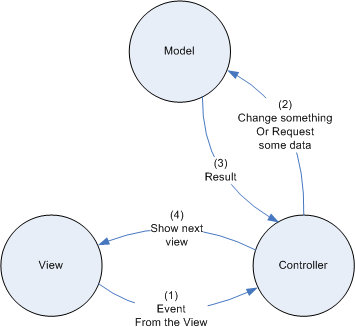
\includegraphics[scale=0.5]{mvcconcept}
\vspace{2mm}

Das Projekt verwendet zudem Singleton-Klassen, um zentrale Funktionalität zu bündeln. Diese werden in sogenannten \emph{Engines} implementiert. Dazu gehören unter anderem Datenbank, Session und Routing.

Es wurde entschieden, ein Index-Rewrite auf dem Webserver zu konfigurieren, um einfachere Pfade verwenden zu können (z.B. \textit{/login} statt \textit{index.php?page=login}) Das Auflösen des Pfades und die Entscheidung, welche MVC Komponenten verwendet werden sollen, übernimmt eine Komponente des \href{https://github.com/steampixel/simplePHPRouter}{steampixel/simplePHPRouter} Frameworks.

\subsection{Datenbank ERM-Diagramm}
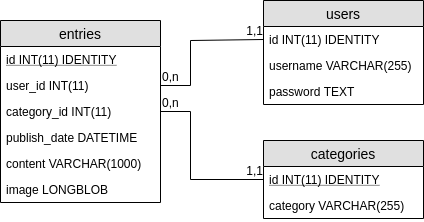
\includegraphics[scale=0.7]{database}

\clearpage
\subsection{Klassendiagramm UML}
Das nachfolgende Klassendiagramm UML zeigt die Struktur des Frameworks auf.

\vspace{2mm}
\mbox{}
\begin{center}
    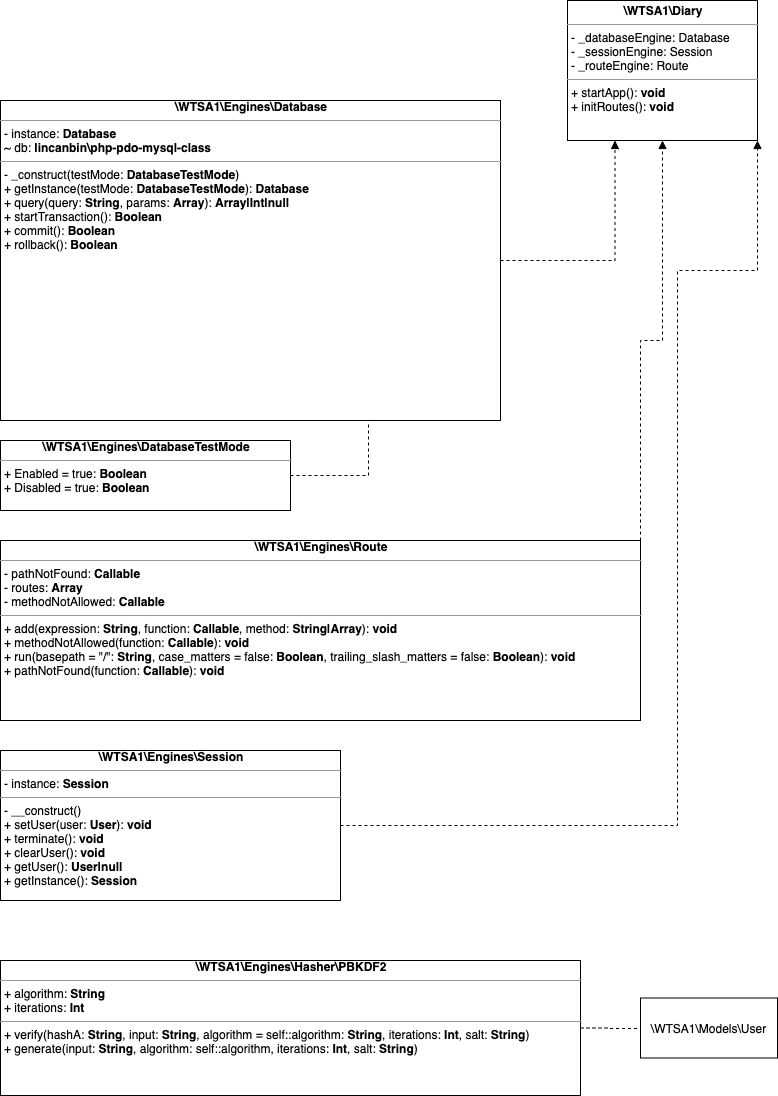
\includegraphics[scale=0.5]{engine_classes.png}
\end{center}

\mbox{}
\begin{center}
    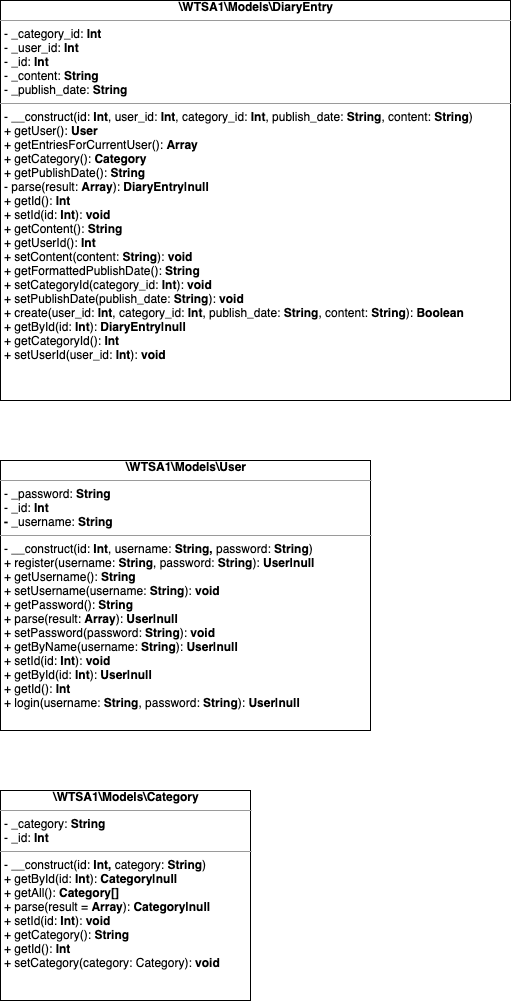
\includegraphics[scale=0.5]{model_classes.png}
\end{center}

\mbox{}
\begin{center}
    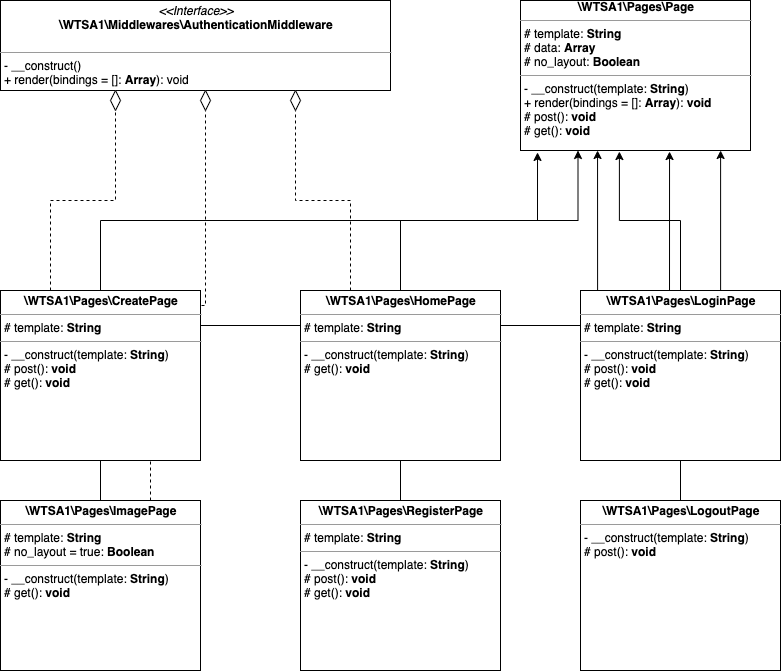
\includegraphics[scale=0.5]{page_classes.png}
\end{center}
\vspace{2mm}


\clearpage
\section{Anhänge}
\subsection{Persönliche Erkenntnisse}
\subsubsection*{Findung Lösungsvariante}
Dank vorhandener Vorerfahrung, war es für eine technisch simple Aufgabe wie dieses Projekt kein grosses Problem, eine relativ optimale Lösung zu finden.

Nach dem Abschluss des Projektmanagement-Workshops steht fest, dass die Voranalyse und Entscheidungsfindung definitiv professioneller und strukturierter hätte ausfallen können.

Es wurde entschieden, diese nicht rückwirkend nachzuarbeiten, da bereits ein nicht unwesentlicher Teil des Projekts implementiert wurde. Stattdessen werden relevante technische Entscheidung in schriftlicher Form im Verlauf dieses Dokuments festgehalten.

\subsubsection*{Sprintplanung Festtage}
Die ursprüngliche Sprintplanung rechnete die Festtage 2019/2020 mit ein.
Es war zwar bewusst, dass dies unter Umständen nicht korrekt funktionieren würde, es wurde aber entschieden, diesen Ansatz trotzdem zu probieren.
Rückblickend, wäre es sinnvoller gewesen, die Festtage grosszügig zu umplanen und dafür den vorherigen und nachfolgenden Sprint ein bisschen dichter zu packen.

\subsection{Externe Verweise}
\begin{itemize}
  \item Öffentliche Repository: \href{https://github.com/ibzti2018/ti3-wt-sa}{github.com/ibzti2018/ti3-wt-sa}
  \item Ausgelieferte Version: \href{https://ibz-wtsa1.dev.cybrox.eu/}{ibz-wtsa1.dev.cybrox.eu}
\end{itemize}


\end{document}
